\section{Sintesi di \ce{[Cr2(OAc)4].2H2O}}
\subsection{Sintesi}
\subsubsection{Procedura sperimentale}

Iniziamo pesando 1.0 g di  bicromato di potassio. Successivamente, pesiamo 5.0 g di zinco polvere e trasferiamo sia il bicromato che lo zinco in un Schlenk precedentemente posto in atmosfera di azoto. In un altro Schlenk, anch'esso in atmosfera di azoto, sciogliamo 4,5 g di \ce{Na(OAc).3H2O} in 4 mL di acqua disareata, scaldando leggermente per ottenere completa dissoluzione. Sotto flusso di azoto abbiamo aggiunto 10 mL di HCl concentrato (12 M) goccia a goccia  nello Schlenk contenente il bicromato e lo zinco.
Lo zinco è cominciato a reagire immediatamente con l’acido liberando idrogeno. Abbiamo continuato l’aggiunta dell’acido, accertandoci di non produrre troppa effervescenza. Abbiamo aspettato per circa 15 minuti finché la soluzione ha smesso di produrre gas e non è diventata di colore blu zaffiro. Giunti a questo punto abbiamo connesso i due contenitori tramite un filtro ad Oliva, accertandosi che in entrambi fosse aperto l'azoto, aiutandosi con un sostengo abbiamo travasato la soluzione di \ce{Cr^{2+}} in quella di acetato. Alla formazione di un solido rosso abbiamo aspettato alcuni minuti per poi immergere il contenitore in un bagno di ghiaccio per una dozzina di minuti.
Infine, abbiamo filtrato il solido su un filtro a colonna in atmosfera di azoto
e l'abbiamo lasciato seccare sotto vuoto per una notte.






\subsubsection{Apparato sperimentale}
L'apparato di sintesi è composto da due tubi Schlenk, un filtro a oliva e un adattatore maschio-maschio\footnote{Quest'ultimo non è presente in figura ma nell'apparato originale era presente.}

Prima si monta un tubo Schlenk vi si pongono le polveri e si fanno un po' di cicli vuoto-azoto. Si bonifica dall'aria anche la sezione che comporrà la parte inferiore dell'apparato tappando l'estremità libera con una valvola analogamente a come fatto con il filtro nella \autoref{sec:cosalenapp}. Successivamente prepariamo la soluzione mantenendo tutto sotto flusso di azoto. Aiutandosi con un sostegno incliniamo entrambi i pezzi fino a raggiungere un posizione quasi orizzontale, sigilliamo e trasferiamo il contenuto del tubo contenente il cromo nella soluzione di acetato. Sotto azoto togliamo il filtro e l'altro tubo e sostituiamo con un tappo. 

Per le operazioni di filtraggio invece procederemo come già visto in \autoref{sec:cosalenapp}.



\begin{figure}[ht!]
    \centering
    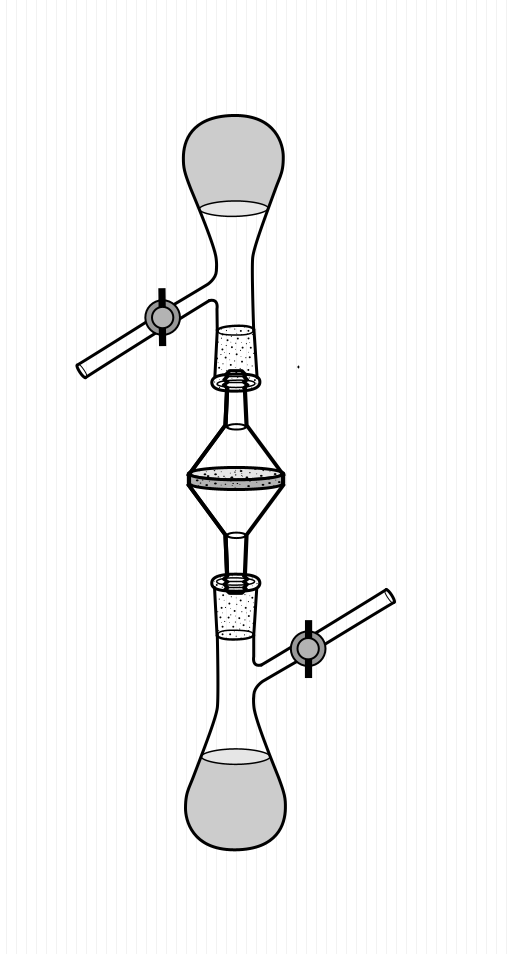
\includegraphics[width=0.3\linewidth]{foto/apparatooliva.png}
    \caption{Schema apparato di sintesi. Anche in questo caso le valvole vanno tenute preferibilmente dalla stessa parte}
    \label{fig:cracetao}
\end{figure}


\subsubsection{Commenti e osservazioni}

Bisogna fare particolare attenzione quando si maneggiano i bicromati in quanto sono molto tossici\footnote{Domanda forse ingenua: perché non abbiamo direttamente usato un sale di cromo(III) che è meno tossico e cancerogeno? In teoria avremo consumato anche meno zinco  \cite{cancer}.}. 
Formazione di un solido rosso dopo l'aggiunta della soluzione di cromo(II) a quella di acetato. 
Il solido asciutto e relativamente stabile all'aria ma comunque si degrada con il tempo. A differenza del cobalto salen in questo caso abbiamo adottato dei tubi Schlenk. Questa è una precauzione necessaria per salvaguardare le linee Schlenk in quanto, durante la reazione avviene la produzione di \ce{H2} che potrebbe creare schiume che sviluppandosi in altezza potrebbero arrivare alle linee dei gas entrando nei tubi e trasportandovi acido. Usando i tubi e aggiungendo cautamente l'acido questa problematica viene risolta.


\subsubsection{Calcoli e analisi dei dati}
In partenza avevamo un numero di moli pari a


\[   n_{\ce{K2Cr2O7}} = \frac{m_{\ce{K2Cr2O7}}}{M_{\ce{K2Cr2O7}}} = \frac{1 \um{g}}{294.19 \um{g/mol}} = 3.40 \um{mmol}\]

\[   n_{\ce{Zn}} = \frac{m_{\ce{Zn}}}{M_{\ce{Zn}}} = \frac{5 \um{g}}{65.41 \um{g/mol}} = 76.4 \um{mmol}\]


Il rapporto stechiometrico 1:2  quindi il notiamo che lo zinco è nettamente in eccesso. La resa verrà calcolata sulle moli di cromato.


Calcoliamo la resa 
\[ Y_\% = \frac{n_\text{pro}}{n_{\ce{Cr2(OAc)4.3H2O}}}\cdot 100 \]

Le moli finali sono il rapporto massa della provettà piena di prodotto tolta la tara e la massa molare del prodotto.

\[ n_\text{pro} = \frac{(m_{f} - m_{t})}{M_\text{pro}} 
 = \frac{ 17.6259 \um{g} - 15.0654 \um{g} }{ 588.40 \um{g/mol}} =  \frac{2.560 \mathrm{~g}}{588.40 \mathrm{~g} / \mathrm{mol}}=3.247 \um{mmol}\]

\[ Y_\% = \frac{n_\text{pro}}{n_{\ce{[Co(en)3]Cl3}}}\cdot 100  = \frac{ \cdot 3.247 \cdot 10^{-3} \mathrm{~mol}}{3.40 \cdot 10^{-3} \mathrm{~mol}} \cdot 100 =95.5\%\]

